\chapter{Mushroom Rock Road}

\begin{enumerate}
	\item \sd, \cs.
	\item Clasko Skip
	      \begin{itemize}
		      \item Run forward to the 3 Soldiers
		      \item Wedge yourself behind the right soldier by holding Left for a second
		      \item Tap Down-Right, X to speak to the bottom soldier
		      \item If the Soldier got away:
		            \begin{itemize}
			            \item Run up near the white spot on the wall near the trigger
			            \item Talk to the Soldier right after he pushes you into the trigger
			            \item Mash until trigger dialogue during the \cs
		            \end{itemize}
	      \end{itemize}
	\item Flee from any encounters, go to the next screen.
	\item \save. Go up the lift. Follow path.
	\item \formation{\tidus}{\wakka}{\auron}
\end{enumerate}
\begin{battle}{Non-Garuda Non-Ambush Anything}
	Try to make it an encounter with a Funguar, but take whatever the third encounter is.
	\begin{itemize}
		\switch{\tidus}{\kimahri}
		\kimahrif Defend
		\wakkaf Defend
		\switch{\auron}{\yuna}
		\summon{\valefor}
		\valeforf Energy Ray
	\end{itemize}
\end{battle}
\begin{equip}
	\begin{itemize}
		\wakkaf Scout/Ice Ball
	\end{itemize}
\end{equip}
\begin{enumerate}[resume]
	\item \formation{\tidus}{\wakka}{\auron}
\end{enumerate}
\vfill
\begin{spheregrid}
	\begin{itemize}
		\yunaf (8 S.Lvl)
		\begin{itemize}
			\item Use Magic Sphere
			\item +4 Magic
			\item Move $\rightarrow\rightarrow\rightarrow\rightarrow$
			\item +3 MagDef, +3 Magic, +20 MP
		\end{itemize}
		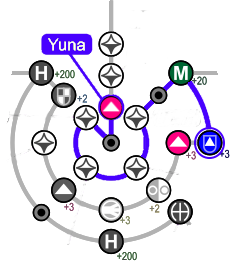
\includegraphics{graphics/Yuna_MRR_1}
		\kimahrif (6 S.Lvl)
		\begin{itemize}
			\item Move $\rightarrow$
			\item +200 HP
			\item Move $\leftarrow\uparrow$
			\item +200 HP
			\item Move $\leftarrow$
			\item +200 HP
		\end{itemize}
		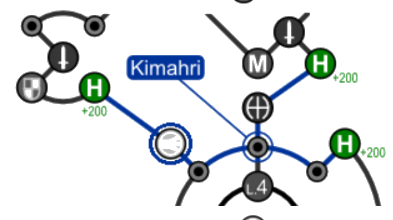
\includegraphics{graphics/kimahrimmr}
		\wakkaf (7 S.Lvl)
		\begin{itemize}
			\item Move $\rightarrow x4 (\downarrow)$Silence Attack
			\item +2 Strength
		\end{itemize}
		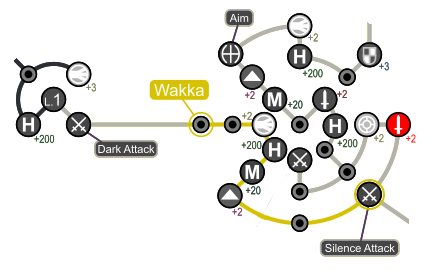
\includegraphics[width=.9\columnwidth]{graphics/Wakka_Grid}
	\end{itemize}
\end{spheregrid}
\vfill
\begin{encounters}
	\begin{itemize}
		\item Raptor, Gandarewa, Red Element
		      \begin{itemize}
			      \switch{\tidus}{\kimahri} if didn't get a Funguar \od, else Defend
			      \kimahrif Defend
			      \wakkaf Attack Raptor
			      \summon{\valefor}
			      \valeforf  Water Gandarewa
			      \valeforf Boost
			      \valeforf Blizzard Red Element
		      \end{itemize}
		\item Raptor, Funguar, Red Element
		      \begin{itemize}
			      \switch{\tidus}{\kimahri} if didn't get a Funguar \od, else Defend
			      \kimahrif Defend
			      \wakkaf Attack Raptor
			      \summon{\valefor}
			      \valeforf  Fire Funguar
			      \valeforf Boost
			      \valeforf Blizzard Red Element
		      \end{itemize}
		\item Raptor, Lamashtu, Red Element
		      \begin{itemize}
			      \switch{\tidus}{\kimahri}
			      \kimahrif  Attack Lamashtu
			      \wakkaf Attack Raptor
			      \switch{\auron}{\yuna}
			      \summon{\valefor}
			      \valeforf Fire Lamashtu
			      \valeforf Boost
			      \valeforf Blizzard Red Element
		      \end{itemize}
		\item Gandarewa, Funguar, Red Element
		      \begin{itemize}
			      \switch{\tidus}{\kimahri} if didn't get a Funguar \od, else Defend
			      \kimahrif Lancet Gandarewa
			      \wakkaf  Attack Gandarewa
			      \switch{\auron}{\yuna}
			      \summon{\valefor}
			      \valeforf Fire Funguar
			      \valeforf Boost
			      \valeforf Blizzard Red Element
		      \end{itemize}
		\item Gandarewa, Lamashtu, Red Element
		      \begin{itemize}
			      \switch{\tidus}{\kimahri}
			      \kimahrif  Attack Lamashtu
			      \wakkaf  Attack Gandarewa
			      \switch{\auron}{\yuna}
			      \summon{\valefor}
			      \valeforf Fire Lamashtu
			      \valeforf Boost
			      \valeforf Blizzard Red Element
		      \end{itemize}
		\item Garuda: Flee
	\end{itemize}
\end{encounters}
\newpage
\begin{enumerate}[resume]
	\item Keep the \formation{\kimahri}{\wakka}{\yuna}
	\item While Yuna still needs AP, do the following
\end{enumerate}
\begin{encounters}
	\begin{itemize}
		\wakkaf Attack Raptors or Gandarewas
		\yunaf Defend
		\item Flee
	\end{itemize}
\end{encounters}
\begin{spheregrid}
	\begin{itemize}
		\yunaf (3 S.Lvl)
		\begin{itemize}
			\item Move $\downarrow\downarrow$
			\item +3 Magic, +3 Agi
		\end{itemize}
		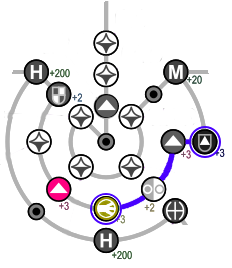
\includegraphics{graphics/Yuna_MRR_2}
	\end{itemize}
\end{spheregrid}
\begin{enumerate}[resume]
	\item \formation{\tidus}{\yuna}{\wakka}
	\item Speak to the man to the left, right before the elevator that brings you up the to HQ Elevator, on the second screen, for 400 Gil. Go on lift, go to HQ.
	\item Walk down and \sd. Walk right to next screen, then right, \sd. Walk right to O'aka
\end{enumerate}
\begin{shop}{10890}
	\begin{itemize}
		\item Sell
		      \begin{itemize}
			      \item Hi-Potions
			      \item X-Potions
			      \item Elixirs
			      \item Hunter's Spear
			      \item Anything other than Longsword, Official Ball, Lightning Steel, Thunder Ball
		      \end{itemize}
		\item Buy
		      \begin{itemize}
			      \item Sentry, Equip
		      \end{itemize}
	\end{itemize}
\end{shop}
\begin{enumerate}[resume]
	\item \save
	\item \sd, go right, \cs[1:00], \sd\ after Seymour. Go down to guard, confirm Yes, \sd
\end{enumerate}
\vfill
\begin{battle}[12000]{Sinspawn Gui 1}
	\begin{itemize}
		\switch{\yuna}{\auron}
		\auronf Power Break Main Body
		\tidusf Defend
		\wakkaf Switch Weapon to Thunder Ball, Power Ball, or Official Ball
		\switch{\wakka}{\kimahri}
		\kimahrif Self Destruct main body
		\switch{\tidus}{\yuna}
		\summon{\valefor}
		\valeforf Energy Blast \od\ x2
		\item \textit{If \valefor\ doesn't charge second \od:}
		      \begin{itemize}
			      \valeforf Shield until Gui used a physical attack
			      \valeforf Boost
			      \valeforf Energy Blast \od
		      \end{itemize}
		\item \textit{If Self Destruct Crit \textit{(7464)}:}
		      \begin{itemize}
			      \valeforf Energy Blast
			      \valeforf Thunder Main Body
		      \end{itemize}
		\item \textit{If Power Break Failed}
		      \begin{itemize}
			      \valeforf Energy Blast
			      \summon{\ifrit}
			      \ifritf Fire Main Body until 3000 HP
			      \ifritf Hellfire
		      \end{itemize}
	\end{itemize}
\end{battle}
\begin{enumerate}[resume]
	\item \cs+\skippablefmv[2:20]. \sd\ Seymour dialogue.
\end{enumerate}
\begin{battle}[6000]{Sinspawn Gui 2}
	\begin{itemize}
		\item \textit{If \yuna\ or \valefor\ don't have \od:}
		      \begin{itemize}
			      \item \textbf{\textcolor{YellowGreen}{Seymour}}: Thundara Head ($\leftarrow$)
			      \item \textbf{\textcolor{YellowGreen}{Seymour}}: Thundara Body x5
			            \yunaf Defend
			            \auronf Defend
		      \end{itemize}
		\item \textit{If they do:}
		      \begin{itemize}
			      \item \textbf{\textcolor{YellowGreen}{Seymour}}: Thundara Body x2
			            \summon{\valefor} or Grand Summon \valefor
			            \valeforf Energy Blast
		      \end{itemize}
	\end{itemize}
\end{battle}
\begin{enumerate}[resume]
	\item \sd, \cs+\skippablefmv[2:00] (press Start immediately after the skip. Do not use it on the upcoming scenes, as you will crash your game). Walk left and up to Gatta, \sd. \fmv+\cs[1:30], \sd\ during \tidus\ monologue. \cs[1:00], \sd
	\item Walk left, \sd. Walk left, speak to \auron, \sd. \save\ if \auron\ is in critical HP. Go up and right, \sd, exit area, \sd.
\end{enumerate}
\vfill
\
\columnbreak

